\documentclass{article}
\usepackage[utf8]{inputenc}
\usepackage[spanish]{babel}
\usepackage{hyperref}
\usepackage{url}
\usepackage{graphics}
\usepackage{subfigure}
\usepackage{amssymb,amsmath,amsthm,amsfonts}
\usepackage{calc}
\usepackage{graphicx}
\usepackage{subfigure}
\usepackage{gensymb}
\usepackage{natbib}
\usepackage{xurl}
\usepackage[utf8x]{inputenc}
\usepackage{amsmath}
\usepackage{graphicx}
\usepackage{parskip}
\usepackage{fancyhdr}
\usepackage{hyperref}
\usepackage{vmargin}
\usepackage{ragged2e}
\setmarginsrb{3 cm}{1.5 cm}{3 cm}{1.5 cm}{1 cm}{1.5 cm}{1 cm}{1.5 cm}

\title{Laboratorio Hash Criptografía}
\author{Diego Carrillo }
\date{Junio 2022}

\begin{document}
\maketitle

\newpage
\tableofcontents
\newpage
\section{Introducción}
En el presente informe, se explicaran los pasos a seguir para desarrollar el laboratorio numero 3 correspondiente al curso de criptografía.En donde, se desarrollará un cifrado creado por el alumno.
\newline \newline
Este cifrado corresponderá a crear un hash para integridad, en donde se ''codificarán'' todos los inputs que sean ingresados.
\section{Hito I}
En primera instancia, se debe de entregar un repositorio en donde se encontraran todos los avances correspondientes en conjunto del código final.
\\\\
\href{https://github.com/Carro1331/Hash}{Repositorio Github @Carro1331}
\\\\
En donde, se toma le decisión de crear un algoritmo para realizar integridad de datos.

\section{Hito II}
Una vez escogido el caso de uso de este algoritmo, se procede a desarrollar el código. Para el cual, se escoge trabajar con Python3, ya que es el lenguaje de programación que se ha utilizado, en su mayoría, durante este curso y a su vez, es el lenguaje mas dominado por el estudiante.
\\\\
Cuando fue el momento de empezar a desarrollar este algoritmo, se empezó teniendo una idea de tomar el string o el texto que fuese recibido por consola o txt y se realizaría un juego de números binarios en conjunto con tablas ASCII. Con las pruebas que se fueron realizando y las situaciones que se fueron analizando, se decide no trabajar con binario, y simplemente realizar un ''codificado'' mediante el uso de tablas ASCII o en otras palabras, se utilizo y creo un hasheo mediante unicode(utf-8). 
\\\\
Una vez claro lo mencionado anteriormente, se empieza con la explicación correspondiente a la actividad. Las funciones se irán explicando según el orden que se mantengan en el código, y no, por el orden que fueron desarrolladas. 
\newpage
\subsection{getUnicode()}
En esta sección, se crea un archivo, donde se registraron los primeros 500 caracteres que pueden ser creados mediantes las funciones de unicode.Para esto, se creó un ciclo de 500 datos en donde se transformó el numero en carácter.
\newline \newline
Esto fue realizado, para poder descubrir de forma manual, cuales fueron los caracteres que producían errores o bien, no eran compatibles del todo con visual estudio code o python3. 

\begin{figure}[h!]
    \centering
    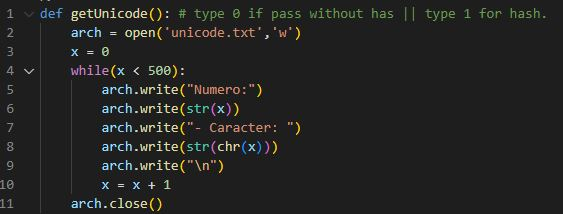
\includegraphics{getunicode.JPG}
    \caption{getUnicode}
    \label{fig:my_label}
\end{figure}

\subsection{getASCII(symbol)}
Esta función, toma el ord() que retorna el valor de un carácter dentro de la tabla ASCII, esta se creó para tener una mayor claridad al momento de utilizar estas funciones, ya que fueron la base para este.

\begin{figure}[h!]
    \centering
    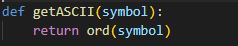
\includegraphics{getascii.JPG}
    \caption{getASCII}
    \label{fig:my_label}
\end{figure}
\newpage
\subsection{encode(string)}
Esta, es la función principal de este programa, en donde se realiza todo el supuesto ''hash''. Para esta función se recibirá un string, la cual simularía la supuesta contraseña, a esta, se le obtendrá el largo en primera instancia para posteriormente ir trabajando con estos valores.
\\\\
Primero, es necesario definir un arreglo con todos los posibles caracteres que no son aceptados por Python o Visual Estudio Code, como se mencionó en las funciones anteriores. Estos valores, se guardan en el arreglo para posteriormente, ir revisando si los caracteres resultantes son o no validos.

\begin{figure}[h!]
    \centering
    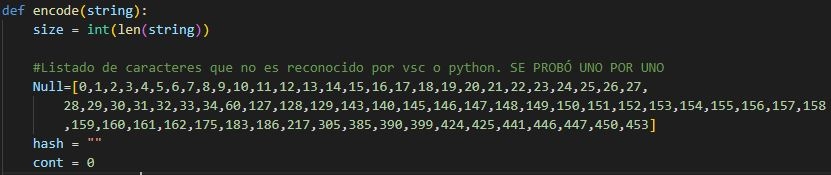
\includegraphics[scale=.7]{encode_list.JPG}
    \caption{encode\_List}
    \label{fig:my_label}
\end{figure}
Una vez realizado el arreglo para evitar los errores, se crean las variables donde se irá guardando el resultado final de este ''codificado'' creado, que tomara el nombre de \textbf{Carro}.
\\\\
Se empieza tomando una par de condicionales, ya que el hash que se deberá crear tiene que tener un largo de 55 caracteres, ni más ni menos. Es por esto, que apenas se reciben los caracteres que el usuario desee ingresar se revisara si es mayor o no al largo deseado. 
\\\\
Si el largo del dato recibido es menor a 55 se procede a ingresar a la condición menor a 55. En donde, se calcula, cuantos son los datos necesarios para llegar a cumplir el largo del hash deseado. 
\\\\
Una vez obtenido este valor, se empiezan a codificar los caracteres que se ingresaron. Esto mediante un ciclo que tendrá una variable \textbf{cont} para ir guardando los valores de la tabla ASCII y se irán sumando con el valor subsecuente, de esta manera se irán codificando los datos.
\\\\
Obtenidos estos datos codificados, se procede a revisar si estos valores se encuentran dentro de la lista creada al comienzo de la función se procede a cambiar este valor sumándole una porción de su propio valor.
\\\\
Como se estuvo trabajando, en primera instancia, con los caracteres que fueron recibidos, es necesario empezar a rellenar los datos restantes, y para esto se fue crearon patrones como ir sumando dígitos dentro de una variable, que se convertirá pasará a la tabla ASCII para luego ir agregándola al hash final. 
\begin{figure}[h]
    \centering
    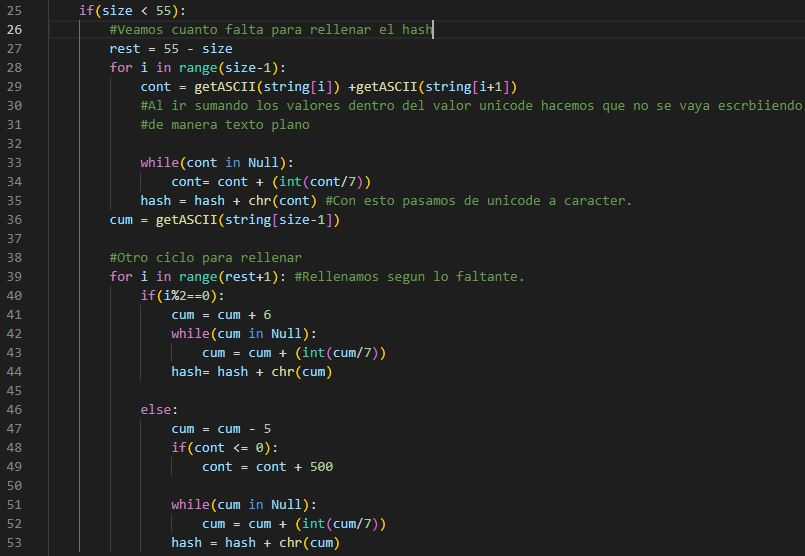
\includegraphics[scale=.65]{ifmenor55.JPG}
    \caption{if menor 55}
    \label{fig:my_label}
\end{figure}
\newpage
Terminada esta condicional, existe el caso contrario, en donde la cantidad de caracteres entregados por el usuario fueron mayores al hash que se realizara. Para esto, es necesario ver primero el largo que estamos trabajando para luego ir seccionándolo, este dividirá en 55 partes donde luego se multiplicará en 55 para tener un estimado de cuantas partes fueron creadas y así estimar un nuevo largo.
\\\\
Se recorrerá el largo estimado y se empezara a crear el hash. en donde existirá una serie de condiciones dentro de este ciclo. Por ejemplo, si la posición que estoy revisando, su siguiente es un espacio vacío se codificara de una manera. En cambio, si no es un extremo, se codificará igual que en la parte anterior, tomando el valor de la tabla ASCII de una posición y sumándole la siguiente. Todo esto, para las sub partes creadas o a analizar en donde se ira concatenando los valores al hash final. 
\\\\ 
En caso contrario, se tomara los valores de la tabla ASCII para la posición que estoy investigando sumada a la siguiente y la resta de la mitad del sucesor. Para finalmente volver a concatenar al hash los resultados obtenidos. 
\\\\
Finalizadas las condiciones, se procede a retornar la palabra hasheada. 
\begin{figure}[h!]
    \centering
    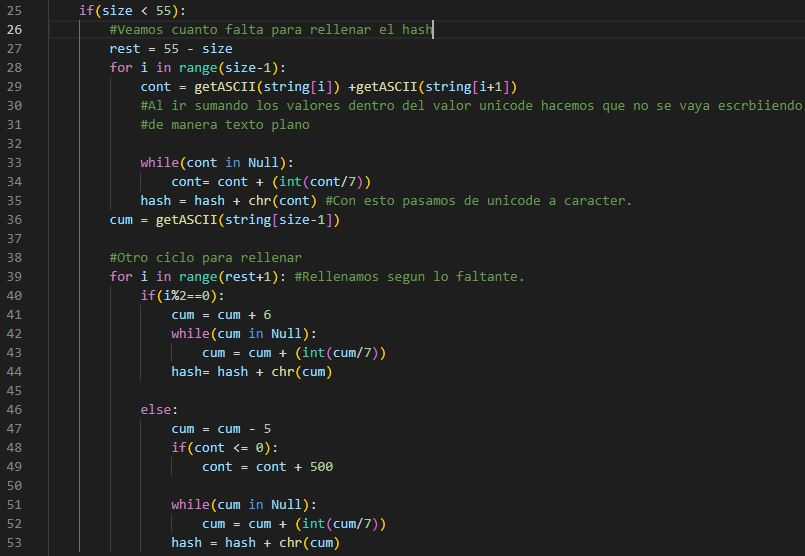
\includegraphics[scale=.7]{ifmenor55.JPG}
    \caption{ifmenor55}
    \label{fig:my_label}
\end{figure}
\newpage

\subsection{writePass(text)}
Esta función fue creada para poder realizar pruebas y generar un registro de los cambios que se fueron creando. 
\begin{figure}[h]
    \centering
    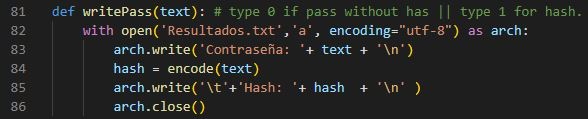
\includegraphics{writepass.JPG}
    \caption{writePass}
    \label{fig:my_label}
\end{figure}

\newpage
\subsection{entropía()}
Al momento de ver la integridad de datos, se puede ver que tan segura puede llegar a ser una contraseña mediante la entropía que puede llegar a poseer esta contraseña. Es por esto que se procede a calcular la entropía.
\\\\
Primero, es importante saber que para calcular la entropía es necesario saber una serie de datos:

\begin{itemize}
    \item El largo de la contraseña
    \item La base del abecedario utilizado
\end{itemize}
Una vez obtenidos estos valores, se crearon condiciones para los casos que se deberá calcular, esto significa crear una condición para cada uno de los casos: 

\begin{itemize}
    \item MD5
    \item SHA1
    \item SHA256
    \item Carro
\end{itemize}

\begin{figure}[h]
    \centering
    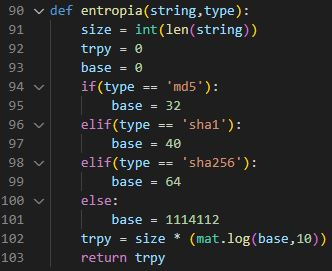
\includegraphics{entropia.JPG}
    \caption{Entropía}
    \label{fig:my_label}
\end{figure}
\newpage
\section{Hash}
En este apartado, se crearon las funciones para obtener los resultados de un hash para cada tipo que sea solicitado, los tipos solicitados fueron los siguientes:
\begin{itemize}
    \item MD5
    \item SHA1
    \item  SHA256
\end{itemize}
Estas funciones, retornan de manera inmediata los hash que se soliciten.
\begin{figure}[h]
    \centering
    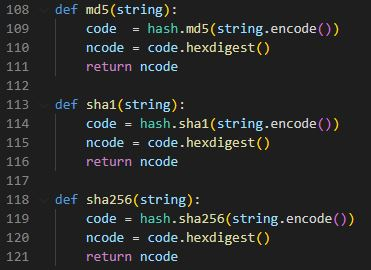
\includegraphics{md5sha1sha256.JPG}
    \caption{Hashs}
    \label{fig:my_label}
\end{figure}

\subsection{leerdatos()}
Como para esta actividad, es necesario leer archivos de texto, en donde se reciben las contraseñas a encriptar, fue necesario crear esta función en donde retornará los datos que se encuentran en el texto. 
\begin{figure}[h]
    \centering
    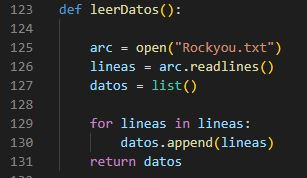
\includegraphics{leerdatos.JPG}
    \caption{leerdatos}
    \label{fig:my_label}
\end{figure}

\subsection{Main}
En esta función, se llamaran todas las funciones que son creadas para luego obtener estos resultados y ponerlos a prueba. Para esto, se empieza creando un ciclo infinito en conjunto de un menú en donde el usuario que quiera utilizar este código, podrá escoger cuantas palabras quiere encriptar, para posteriormente ir recibiendo los valores de la entropía y los tiempos de ejecución.
\\\\
Las opciones para trabajar con este programa es trabajar con 1, 10, 20 o 50 palabras a encriptar. En donde se empezarán a agregar a una lista enlazada las palabras que se desean utilizar. Para luego, empezar a recorrer esta lista mientras se están tomando los tiempos por cada encriptado que se esta realizando. Y los tiempos se irán guardando dentro de listas para luego mostrarlas por pantalla.
\begin{figure}[h]
    \centering
    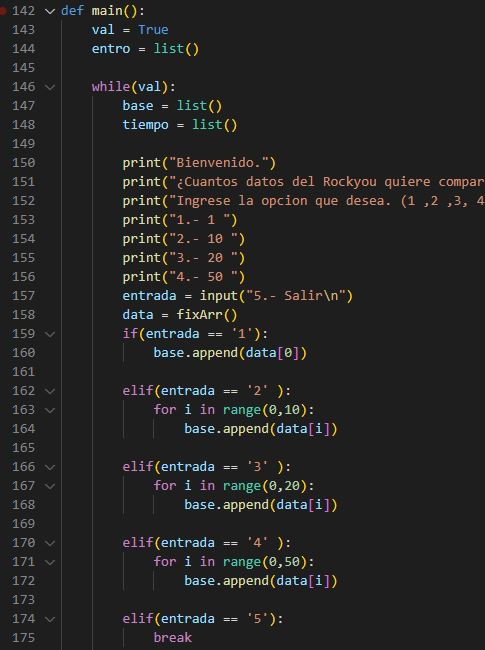
\includegraphics{main1.JPG}
    \caption{main1}
    \label{fig:my_label}
\end{figure}

\begin{figure}[h]
    \centering
    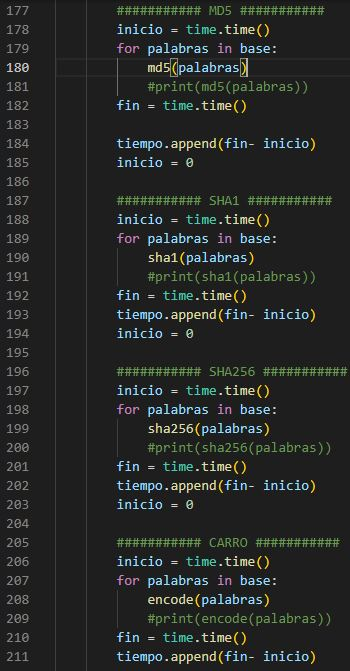
\includegraphics{maintiempos.JPG}
    \caption{tiempos}
    \label{fig:my_label}
\end{figure}

\begin{figure}[h]
    \centering
    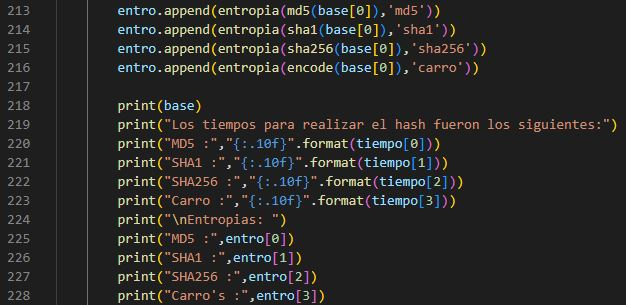
\includegraphics{output.JPG}
    \caption{output}
    \label{fig:my_label}
\end{figure}
\newpage

\end{document}
